\begin{surferPage}[Kummers-flaten]{Kummers flate av fjerde grad}
	I 1875 var Eduard Kummer den første til å stille spørsmålet om det maksimale antallet singulariteter til en flate av fjerde grad.
 	
	Han viste at antallet var $16$, det vil si at $\mu(4)=16$. Deretter gjorde han detaljerte 
	studier av flater av fjerde grad med $16$ singulariteter. En spesielt vakker familie av slike flater er gitt ved:
		
    \[\bigl(x^2+y^2+z^2-\mu^2\bigr)^2 - \lambda
    \,y_0\,y_1\,y_2\,y_3,\]
	
    hvor $\mu$ er en fri parameter, og 
    $\lambda = \frac{3\mu^2-1}{3-\mu^2}$;. $y_i$ er sidene til det vanlige tetraederet 
	{\small
	
    $y_0=1-z-\sqrt{2}x$, \  
    $y_1=1-z+\sqrt{2}x$, \ 
    $y_2=1+z+\sqrt{2}y$, \ 
    $y_3=1+z-\sqrt{2}y$}
	
  for å gjøre flaten symmetrisk. Ikke alle medlemmene av denne familien har akkurat $16$ reelle 
  singulariteter, selv om de fleste av dem har det:
  \begin{center}
    \vspace*{-0.2cm}\hspace*{-0.2cm}
    \begin{tabular}{@{}c@{\,}c@{\,}c@{\,}c@{\,}c@{}}
      \begin{tabular}{@{}c@{}}
        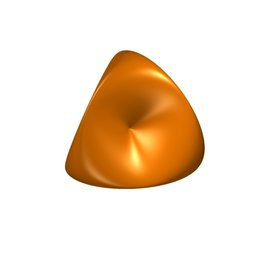
\includegraphics[height=1.4cm]{./../../common/images/kummer_0}
      \end{tabular}
      &
      \begin{tabular}{@{}c@{}}
        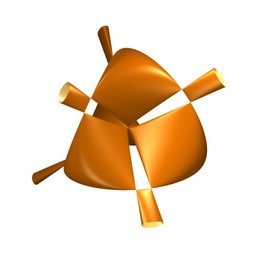
\includegraphics[height=1.4cm]{./../../common/images/kummer_1}
      \end{tabular}
      &
      \begin{tabular}{@{}c@{}}
        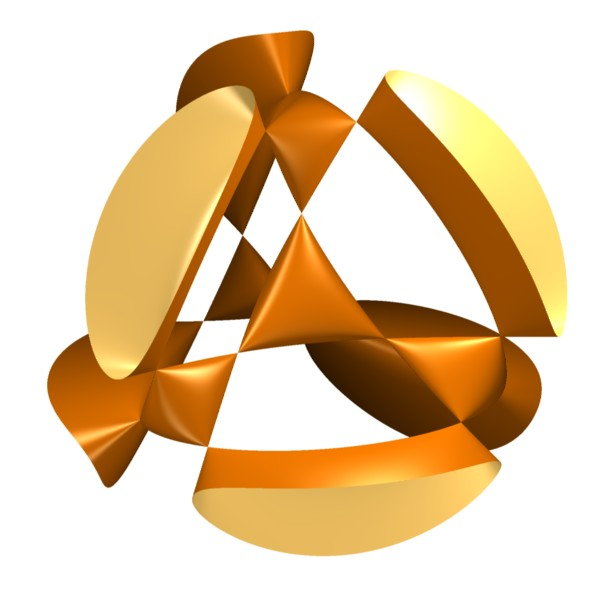
\includegraphics[height=1.4cm]{./../../common/images/kummer_2}
      \end{tabular}
      &
      \begin{tabular}{@{}c@{}}
        
\includegraphics[height=1.4cm]{./../../common/images/kummer_3}
      \end{tabular}
    \end{tabular}
  \end{center}
  \vspace{-0.2cm}  
  For noen spesielle parameterverdier, kan flere av singularitetene slå seg sammen.
\end{surferPage}
